\section{Inference}
\label{sec:inference}

Now that we have defined the FFBM, we wish to leverage it to perform inference. Suppose we are presented with a vertex-labelled graph $(A, X)$; the goal is to draw samples for $\theta$ according to the posterior given the observed data:
%
\begin{equation}
	\label{eqn:theta-target}
	\theta^{(t)} \sim p(\theta | A, X)
\end{equation}
%
However, generating these samples is not easily done in practice. We therefore propose an iterative approach. We first draw samples $b^{(t)}$ from the block membership posterior (equation \ref{eqn:b-samples}) and then use each $b^{(t)}$ to draw samples for $\theta$ as in equation \ref{eqn:theta-samples}. 
%
\begin{align}
	b^{(t)} &\sim p \Big( b | A, X \Big)  \label{eqn:b-samples}\\
	\theta^{(t)} &\sim p\Big(\theta | X, b^{(t)} \Big) \label{eqn:theta-samples}
\end{align}
%
Both of these sampling steps can be implemented with a Markov Chain through the Metropolis-Hastings algorithm \cite{hastings-alg}. We just need to define a proposal distribution $q(x, x')$ for proposing a move $x \rightarrow x'$ and be able to evaluate an un-normalised form of the target distribution, denoted $\pi(\cdot)$, point-wise. The proposed move is then accepted with probability $\alpha$ (equation \ref{eqn:mh-accept}) else it is rejected and we stay at $x$.
%
\begin{equation}
	\alpha(x, x') = \min \left( \frac{\pi(x') q(x', x)}{\pi(x) q(x, x')} , 1 \right)
	\label{eqn:mh-accept}
\end{equation}
%
This accept-reject step ensures the resulting Markov Chain is in detailed balance with the target distribution $\pi(\cdot)$. What we propose in equations \ref{eqn:b-samples} and \ref{eqn:theta-samples} is therefore implemented through a 2-level Markov chain. The resulting samples for $\theta^{(t)}$ are unbiased in the sense that the expectation of their distribution is the posterior we are targetting:
%
\begin{equation}
\Expect_{b^{(t)}} \left[p \left( \theta | X, b^{(t)} \right) \right] = \sum_{b \in [B]^N} p(\theta | X, b) p(b | A, X) = \sum_{b \in [B]^N} p(\theta, b | A, X) = p(\theta | A, X)
\label{eqn:theta-unbiased}
\end{equation}
%
This is an example of a pseudo-marginal approach. Indeed, \citet{pseudo-marginal} show that the unbiased result in equation \ref{eqn:theta-unbiased} is sufficient to prove that for large enough $t$, $\theta^{(t)} \sim \Expect_{b^{(i)}} \left[ p(\theta | X, b^{(t)})\right] = p(\theta 
| A, X)$ which is exactly the distribution we are targetting (equation \ref{eqn:theta-target}).
%
\begin{figure}[!h]
	\centering

	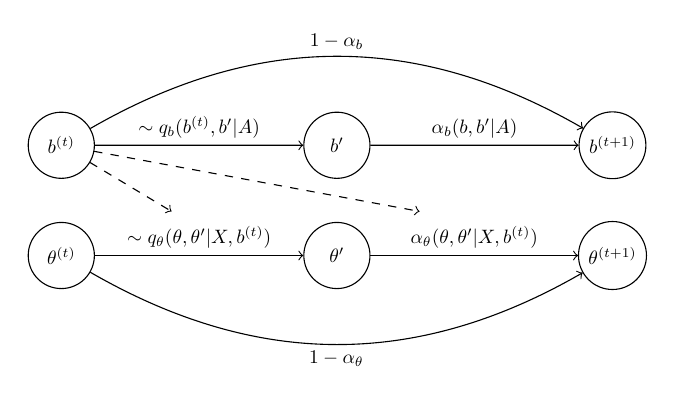
\begin{tikzpicture}[
		scale=0.7, every node/.style={transform shape},
		roundnode/.style={circle, draw=black, minimum size=12mm},
		squarednode/.style={rectangle, draw=black, minimum size=12mm}
		]
		% nodes
		\node[roundnode] (b0) at (0, 2) {$b^{(t)}$};
		\node[roundnode] (b1) at (5, 2) {$b'$};
		\node[roundnode] (b2) at (10, 2) {$b^{(t+1)}$};
		\node[roundnode] (t0) at (0, 0) {$\theta^{(t)}$};
		\node[roundnode] (t1) at (5, 0) {$\theta'$};
		\node[roundnode] (t2) at (10, 0) {$\theta^{(t+1)}$};
		
		% arrows
		\draw[->] (b0) to node[above] {$\sim q_b(b^{(t)}, b' | A)$} (b1);
		\draw[->] (b1) to node[above] {$\alpha_b (b, b' | A)$} (b2);
		\draw[->] (b0) [out=30, in=150] to node[above] {$1-\alpha_b$} (b2);
		
		\draw[->] (t0) to node[above] {$\sim q_\theta(\theta, \theta' | X, b^{(t)})$} (t1);
		\draw[->] (t1) to node[above] {$\alpha_\theta (\theta, \theta' | X, b^{(t)})$} (t2);
		\draw[->] (t0) [out=-30, in=-150] to node[below] {$1-\alpha_\theta$} (t2);
		
		\draw[dashed, ->] (b0) to (2, 0.8);
		\draw[dashed, ->] (b0) to (6.5, 0.8);
		
	\end{tikzpicture}
	\caption{Sampling sequence}
	\label{fig:samp-sequence}
\end{figure}

The reason we split the Markov chain into two stages is because the summation over all latent states $b \in [B]^N$ required to directly compute the likelihood $p(A| X, \theta) = \sum_{b \in [B]^N} p(A | b) P(b | X, \theta)$ is intractable -- $O(B^N)$. Figure \ref{fig:samp-sequence} shows an overview of the proposed method. We have introduced subscripts and conditionings to make explicit what variables each step utilises. We note the power of the simplification given by equation \ref{eqn:b-pseudo-prior}. As $p(b| X)$ does not depend on the exact value of X, we do not need to know the value of $X$ to perform the sampling on $b$. Conversely, for the $\theta^{(t)}$ samples, we use only $b^{(t)}$ but not $A$ as $(\theta \indep A) | b$.

\FloatBarrier

\subsection{Sampling block memberships}

\citet{Peixoto-MCMC} proposes a Monte Carlo method which we will base our approach on. It relies on writing the posterior in the following form:
%
\begin{equation}
	p(b | A, X) \propto p(A | b, X) \cdot p(b | X) = \pi_b(b)
\end{equation}
%
Now $\pi_b(\cdot)$ is the un-normalised density we wish to sample from for the $b$-chain. In other words, we wish to construct a Markov chain that has $\pi_b(\cdot)$ as its invariant distribution. We can break $\pi_b$ down as follows:
%
\begin{equation}
	\pi_b(b) = p(b|X) \sum_{\psi} \nolimits p(A , \psi | b, X) \\
	= p(b|X) p(A, \psi^* | b, X) \\
	= p(A | b, \psi^*) \cdot p(\psi^* | b) \cdot p(b | X)
\end{equation}
%
Since we are using the microcanonical SBM formulation, there is only one value of $\psi$ that is compatible with the given $(A, b)$ pair (given in equation \ref{eqn:sbm-constraints}). We denote this value $\psi^* = \{\psi_k^*, \psi_e^*\}$. Therefore, the summation over all $\psi$ reduces to just the single $\psi^*$ term; this is the power of the microcanonical formulation. We also define the microcanonical entropy of the configuration as.
%
\begin{equation}
	S(b) = - \log \pi_b(b) = - \Big( \log p(A | b, \psi^*) + \log p(\psi^*, b | X) \Big)
	\label{eqn:dl-form}
\end{equation}
%
This entropy can equally be thought of as the description length of the graph. The exact form of the proposal $q_b$ is explored thoroughly by \citet{Peixoto-MCMC} and not repeated here. There is a widely used library for Python made available under LGPL called \verb*|graph-tool| \cite{peixoto_graph-tool_2014}, which implements this algorithm. The only modification we make is in the block membership prior $p(b)$ which we replace with $p(b|X)=B^{-N}$, which cancels out in the MH accept-reject step as it is independent of $b$.

\subsection{Sampling feature-to-block generator parameters}

The invariant distribution we wish to target for the $\theta$ samples is the posterior of $\theta$ given the values of the pair $(X, b)$. We write this as follows:
%
\begin{equation}
	\pi_\theta(\theta) \propto p(\theta | X, b) \propto p(b | X, \theta) p(\theta) \propto \pi_\theta (\theta) \propto  \exp \left( - U(\theta) \right)
\end{equation}
%
Where we have introduced $U(\theta)$ equal to the negative log posterior. We define $y_{ij} \coloneqq \one \left\{ b_i = j \right\}$ and $a_{ij} \coloneqq \phi_j(x_i; \theta)$. Discarding constant terms, we can write $U(\theta)$ as in equation \ref{eqn:U-form} (refer to appendix \ref{appdx:form-U} for the derivation).
%
\begin{equation}
	U(\theta) = \left( \sum_{i=1}^{N} \sum_{j=1}^{B} y_{ij} \log \frac{1}{a_{ij}} \right)
	+ \frac{1}{2\sigma_\theta^2} ||\theta||^2 = N \cdot \Lcal(\theta) + \frac{1}{2\sigma_\theta^2} ||\theta||^2
	\label{eqn:U-form}
\end{equation}
%
$U(\theta)$ in equation \ref{eqn:U-form} appears a typical objective function for neural network training. The first term is introduced by the likelihood. We collect it into $N \cdot \Lcal(\theta)$, which is the cross-entropy between the graph-predicted and feature-predicted block memberships summed over all vertices. The second term of equation \ref{eqn:U-form} -- introduced by the prior -- brings a form of regularisation, guarding against over-fitting. Different to traditional applications, our goal is not to find the minimiser of $U(\theta)$ but to draw samples from the posterior $\pi_\theta(\cdot) \propto \exp(-U(\cdot))$. We can use $\nabla U$ as a useful heuristic to bias our proposal towards regions of higher target density. We therefore adopt the Metropolis-adjusted Langevin algorithm (MALA) -- first proposed by \citet{mala-tweedie}. Given the current sample $\theta$, we generate a new sample $\theta'$ according to equation \ref{eqn:theta-update}.
%
\begin{align}
	\theta' &= \theta - h \nabla U(\theta) + \sqrt{2h} \cdot \xi
	\label{eqn:theta-update} \\
	\therefore q_\theta(\theta, \theta') &= \Gaussian \left( \theta' ; \theta - h \nabla U(\theta), 2h I \right)
	\label{eqn:theta-proposal}
\end{align}
%
Where $\xi \sim \Gaussian(0, I)$ and $h$ is a step-size parameter -- which may vary with the sample index (appendix \ref{appdx:step-size} explores this more fully). Without the injected noise term, MALA is equivalent to gradient descent. We require the noise term $\xi$ to fully explore the parameter space. We can write the proposal distribution $q_\theta$ as in equation \ref{eqn:theta-proposal}. The term $\nabla U$ has an easy to compute analytic form (derived in Appendix \ref{appdx:gradu}). By noting that $\theta = \{w_k\}_{k=1}^{B}$, we write the derivative with respect to each $w_k$ as:
%
\begin{equation}
	\frac{\partial U}{\partial w_k} = - \left( \sum_{i=1}^{N} \Big\{ \tilde{x}_i (y_{ik} - a_{ik}) \Big\} - \frac{w_k}{\sigma_\theta^2} \right)
	\label{eqn:U-derivative}
\end{equation}
%
After a proposed move is generated, in typical Metropolis-Hastings fashion we accept the move with probability $\alpha_\theta$, as in equation \ref{eqn:mh-accept}.

\subsection{Sampling sequence}

Up to this point, each $\theta^{(t)}$ update uses its corresponding $b^{(t)}$ sample. This means that the evaluation of $U(\theta)$ and $\nabla U(\theta)$ has high variance. This may lead to longer burn-in for the resulting Markov chain. The only link between $b^{(t)}$ and $\theta^{(t)}$ is in the evaluation of $U(\theta)$ and $\nabla U(\theta)$ which depends only on the matrix $y^{(t)}$ with entries $y_{ij}^{(t)} \coloneqq \one\{b_i^{(t)} = j\}$. We would rather deal with the expectation of each $y_{ij}^{(t)}$:
%
\begin{equation}
	\Expect \left[ y_{ij}^{(t)} \right] = \Expect_{b^{(t)}} \left[ \one(b_{i}^{(t)} = j) \right]
	= p(b_i = j | A, X)
\end{equation}
%
We can obtain an unbiased estimate for this quantity using the set of $b$-samples. However, as with all MCMC methods, we must only uses samples after burn-in and thinning have been applied. We introduce $\Tcal_b$ to denote the retained set of indices for the $b$-samples and $\Tcal_\theta$ similarly for the $\theta$-chain. An in-depth discussion of how these sets are chosen is given in appendix \ref{appdx:burn-in-thinning}. The unbiased estimate for $y_{ij}^{(t)}$ using the restricted sample set $\Tcal_b$ is denoted $\hat{y}_{ij}$ and has form:
%
\begin{equation}
	\hat{y}_{ij} \coloneqq \frac{1}{|\Tcal_b|} \sum_{t \in \Tcal_b} y_{ij}^{(t)} = \frac{1}{|\Tcal_b|} \sum_{t \in \Tcal_b} \one\{b_i^{(t)} = j\}
\end{equation}
%
We choose to feed each $\theta^{(t)}$ update step the same matrix $\hat{y}$ for all $t$ rather than the corresponding $y^{(t)}$. This means we no longer need to run the $b$ and $\theta$ Markov chains concurrently. Instead, we run the $b$-chain to completion and use it to generate $\hat{y}$. This affords us the flexibility to vary the lengths of the $b$ and $\theta$-chains. Furthermore, the changeover from $y^{(t)}$ to $\hat{y}$ reduces the burn-in time for the $\theta$-chain by reducing the variance in our evaluation of $U$ and $\nabla U$. A description of the overall algorithms is given in appendix \ref{appdx:algorithms}.

\subsection{Dimensionality reduction}
\label{sec:dim-reduction}

Once we have the samples $\left\{ \theta^{(t)} \right\} \sim p(\theta | A, X)$, we can compute the empirical mean and standard deviation of each component of $\theta$. Switching back to matrix notation we define $\theta = W$, such that $W_{ij}$ is the weight component for block $i$ and feature $j$, we can define:
%
\begin{equation}
	\hat{\mu}_{ij} \coloneqq \frac{1}{|\Tcal_\theta|} \sum_{t \in \Tcal_\theta} W_{ij}^{(t)} \qquad \textrm{and} \qquad
	\hat{\sigma}_{ij} \coloneqq \frac{1}{|\Tcal_\theta|} \sum_{t \in \Tcal_\theta} \left( W_{ij}^{(t)} - \hat{\mu}_{ij} \right)^2
\end{equation}
%
A simple heuristic to discard the least important features requires specifying a cutoff $c > 0$ and a multiplier $k > 0$. We define the function $\Fcal_i(j)$ as in \ref{eqn:fij} then only keep features with indices $d \in \Dcal'$, where $\Dcal'$ is constructed as in equation \ref{eqn:kept-feature-set}.
%
\begin{align}
	\Fcal_i(j) &\coloneqq (\hat{\mu}_{ij} - k \hat{\sigma}_{ij}, \hat{\mu}_{ij} + k \hat{\sigma}_{ij}) \cap (-c, +c)
	\label{eqn:fij} \\
	\Dcal' &\coloneqq \left\{ j \in [D] : \exists i \in [B] \textrm{ s.t. }  \Fcal_i(j) \neq \emptyset \right\}
	\label{eqn:kept-feature-set}
\end{align}
%
Intuitively, this means discarding any feature for which $\hat{\mu}_{ij} \pm k\hat{\sigma}_{ij}$ lies within or spans the null region $(-c, c)$ for all block indices. If we were to use the Laplace approximation for the posterior $p(W_{ij} | A, X) \approx \Gaussian(W_{ij}; \mu_{ij}, \sigma_{ij})$, then this is effectively a hypothesis test on the value of $W_{ij}$ (equation \ref{eqn:hyp-test-discard}). $\Dcal'$ then comprises all features $i$ for which $H_1$ is accepted at least once for some $j \in [B]$.
%
\begin{equation}
	H_0: |W_{ij}| \leq c \qquad
	H_1: |W_{ij}| > c
	\label{eqn:hyp-test-discard}
\end{equation}
%
The multiplier $k$ determines the degree of significance of the result. However, as the Laplace approximation is not exact we will only treat this dimensionality reduction method as a useful heuristic and not an exact method. Conversely, we could fix $k=k_0$ and the dimension of our reduced feature set $|\Dcal'|=D'$. We would then like to find the largest value of $c$ such that $|\Dcal'|=D'$ given $k=k_0$. This is summarised in equation \ref{eqn:c-star}. This approach is often preferred as it fixes the number of reduced dimensions.
%
\begin{equation}
	c^* = \argmax_{c>0} (c : |\Dcal'| = D', k=k_0)
	\label{eqn:c-star}
\end{equation}
%
For an algorithmic implementation of this method refer to appendix \ref{appdx:algorithms}.